\chapter{Instalace a oživení systému}

\section{Platforma}

Systém Retrobi je {\em centralizovaný}. Jeho centrálním prvkem je {\em server}, ke kterému se připojují klienti pomocí HTTP. Klienty se zde rozumí jednoúčelové {\em aplikace pro import dat} (připojují se přímo k databázi) a návštěvnící ze sítě internet (připojují se k webové aplikaci). Celý systém je multiplatformní, ale otestován je pod systémem Ubuntu Linux (server) a Windows (klienti).

\subsection{Hardware}

Minimální konfigurace serveru je sestava se dvěma procesorovými jádry na 2~GHz (64~bit), 2~GiB paměti RAM a diskové pole 2~TiB (pro cca 1,5 milionu lístků s rezervou). Na této konfiguraci současně běží databázový, vyhledávací i webový server. V dokumentaci se dále předpokládá tato minimalistická varianta, ačkoliv by bylo teoreticky možné jednotlivé součásti oddělit a po korektní změně nastavení je provozovat na několika fyzicky oddělených strojích.

Výkon celého systému je závislý především na rychlosti přístupu na pevný disk. Doporučujeme proto využít např. technologie RAID, a to i kvůli vyšší spolehlivosti a odolnosti proti ztrátě dat. Další významné zvýšení výkonu by přinesl přechod na technologii SSD (solid state drive). Takový disk by byl zajímavý zejména pro umístění indexů vyhledávacího enginu, které nejsou příliš velké, ale na druhou stranu často využívané. 

Jakoukoliv paměť RAM navíc je možno využít pro zvýšení maximální velikosti haldy (heap size) pro Java Virtual Machine (JVM). Doporučená velikost haldy pro webový server je 2~GiB. Velikost haldy a další možnosti virtuálního stroje se specifikují v souboru {\bf /etc/default/tomcat7} touto konfigurační direktivou:

\begin{verbatim}
JAVA_OPTS="-Djava.awt.headless=true -Xmx2g -XX:+UseConcMarkSweepGC"
\end{verbatim}

\section{Automatická instalace}

Skript pro automatickou instalaci systému Retrobi nám laskavě posytl pan Mgr.~Martin~Krsek. Zabalený skript a jeho součásti naleznete v repositáři SVN v podadresáři {\bf install}. Pro použití skriptu celou tuto složku nakopírujte na server, kde chcete systém Retrobi nainstalovat. Poté spusťte hlavní skript. Ten provede veškerou instalaci, konfiguraci a kompilaci systému Retrobi, takže již stačí jen spustit potřebné systémové služby a provést deploy webové aplikace do serveru Tomcat (viz následující kapitoly). Balíček WAR potřebný pro deploy se nachází ve složce {\bf /opt/RETROBI}. Během běhu skriptu vzniknou logy s ladícími informacemi.

\section{Manuální instalace}

{\bf Poznámka:} Toto je doporučený postup instalace. Pokud jste zkušený administrátor a víte co děláte, můžete samozřejmě instalaci a konfiguraci provést jinak, než je zde uvedeno.

K instalaci systému Retrobi není třeba žádných speciálních programátorských znalostí, ale provádět by ji měl spíše zkušenější správce. K instalaci je potřeba internetové připojení, možnost získat rootovská oprávnění ({např. příkazem {\bf sudo}}), schopnost editovat textové soubory a obecně pracovat se soubory na disku (kopírovat, přesouvat, mazat, vytvářet). Správce musí znát základy práce s terminálem. Znalost všech příkazů ale není nutná, ty jsou popsány v dokumentaci.

Také se předpokládá znalost principů systémových oprávnění a jejich změny, například pomocí příkazů {\tt chmod} a {\tt chown}.

\subsection{Operační systém}

Základem systému Retrobi je operační systém Linux v distribuci Ubuntu (edice Server). Otestována byla verze {\bf 11.10} (64~bit). Tu lze stáhnout z tého adresy:

{\bf http://www.ubuntu.com/download/server/download}

Operační systém se nainstaluje standardním způsobem, není nutné nic speciálního nastavovat. Po instalaci operačního systému je třeba zprovoznit připojení k internetu (mimo rozsah této dokumentace). Připojení většinou proběhne automaticky, pokud je server připojen do sítě s DHCP serverem.

\subsection{Potřebné balíčky}

Verze uvedené u balíčků nejsou přesné a závazné, ale minimální možné. Automatické aktualizace operačního systému Ubuntu zajistí, že budou vždy použity nejnovější verze se všemi dostupnými opravami chyb a vylepšeními. Číslování verzí je hierarchické. To například znamená, že program verze 1 může být aktualizován na verzi 1.0.1, poté na 1.1 a nakonec na verzi 1.2.5. Pokud vyjde verze 2, nemusí být zpětně kompatibilní. Toto ale posuzuje správce balíčků (na straně Ubuntu), který se stará o jejich bezproblémovou aktualizaci a kompatibilitu.

Nejprve doporučujeme nainstalovat správce souboru {\bf mc} (Midnight Commander), který umožňuje procházet disk i editovat textové konfigurační soubory (klávesa F4). Dále je nutné nainstalovat {\bf OpenJDK} pro Javu~1.6, servletový kontejner {\bf Apache~Tomcat}, databázi {\bf CouchDB}, poštovní (e-mailový) server {\bf Postfix}, buildovací systém {\bf Maven} a systémy pro správu verzí {\bf Subversion} a {\bf Git}.

\begin{enumerate}
\item{\bf sudo apt-get install mc maven2 subversion git}
\item{\bf sudo apt-get install openjdk-6-jdk tomcat7-admin}
\item{\bf sudo apt-get install couchdb postfix python}
\end{enumerate}

Otestované verze:

\begin{itemize}
\item{OpenJDK~1.6.b23}
\item{Apache~Tomcat~7.0.23}
\item{CouchDB~1.0.1}
\item{Postfix~2.8.7}
\item{Maven~2.2.1}
\item{svn~1.6.12}
\item{git~1.7.1}
\item{Python~2.3}
\end{itemize}

\subsection{Adresářová struktura}

Pro vyšší přehlednost je vhodné připravit adresáře uvedené v tabulce~\ref{tab:dirs} a zajistit, aby k nim odpovídající aplikace měly potřebná oprávnění pro zápis. Je možné využít symlinků a jednotlivé adresáře umístit na jiné fyzické disky či stroje. V tabulce jsou uvedeny jednotlivé adresáře a jejich předpokládaná velikost po naplnění všemi daty. Proto rozvažte, na který disk který soubor umístíte.

\begin{table}
\centering
\begin{tabular}{|c|c|c|c|}
\hline
Adresář & Zkratka & Zapisující aplikace & Odhad velikosti \\
\hline
\hline
data CouchDB & CESTA\_DB\_DATA & CouchDB & 2~TiB \\
\hline
indexy pro Lucene & CESTA\_INDEX & CouchDB-Lucene & 5~GiB \\
\hline
CSV logy & CESTA\_CSV & webová aplikace & 1~GiB \\
\hline
konfigurační soubory & CESTA\_CONFIG & webová aplikace & 1~MiB \\
\hline
\end{tabular}
\caption{Tabulka adresářů a jejich velikostí}
\label{tab:dirs}
\end{table}

\section{Konfigurace}

\subsection{Databáze CouchDB}

Databáze CouchDB se konfiguruje souborem, který je standardně umístěný na cestě {\bf /etc/couchdb/local.ini} (pozor, druhý soubor {\bf default.ini} obsahuje výchozí konfiguraci a je přepsán při každé aktualizaci CouchDB). V souboru {\bf local.ini} je třeba nastavit tyto parametry:

\begin{verbatim}
[couchdb]
database_dir = CESTA_DB_DATA
view_index_dir = CESTA_DB_DATA
os_process_timeout = 1800000
delayed_commits = false
[httpd]
bind_address = 0.0.0.0
[couch_httpd_auth]
require_valid_user = false
[log]
file = CESTA_DB_DATA/couchdb.log
level = error
[external]
fti=/usr/bin/python CESTA_LUCENE/tools/couchdb-external-hook.py
[httpd_db_handlers]
_fti = {couch_httpd_external, handle_external_req, <<"fti">>}
\end{verbatim}

Databázový server CouchDB je dále nutné zabezpečit např. firewallem tak, aby se k němu nemohl připojit žádný klient kromě vybraných počítačů, na kterých budou provozována \uv{udělátka} a webová aplikace (většinou není nutné speciálně řešit, protože webová aplikace běží na stejném stroji -- {\em localhost}).

\subsection{Vyhledávací servlet CouchDB-Lucene}

Vyhledávací servlet se konfiguruje pomocí {\bf .ini} souboru, který se nachází na tomto umístění:

\begin{verbatim}
retrobisrc/couchdb-lucene/src/main/resources/couchdb-lucene.ini
\end{verbatim}

Před kompilací vyhledávacího servletu CouchDB-Lucene je v něm potřeba nastavit tyto parametry:

\begin{verbatim}
[lucene]
# cesta k vyhledavacim indexum
dir=CESTA_INDEX
# maximalni doba dotazu [ms]
# (nastavime na 30 sekund)
timeout=30000
# vychozi limit na pocet vysledku
limit=10
[local]
# zakladni URL databaze CouchDB
url=http://localhost:5984/
\end{verbatim}

\subsection{Server Tomcat}

Ve výchozím nastavení je server Tomcat možná až příliš \uv{upovídaný} a podrobně loguje různé akce a přístupy. Aby do budoucna nebyl problém s nedostatkem místa na systémovém disku, je doporučeno snížit podrobnost logování a to v tomto souboru:

\begin{verbatim}
/etc/tomcat7/server.xml
\end{verbatim}

Stačí vyhledat a zakomentovat XML uzel {\em Valve} souvisejicí s logováním přístupů (access log), který se nachází pod uzlem {\em Host}:

\begin{verbatim}
<Host name="localhost" appBase="webapps" 
      unpackWARs="true" autoDeploy="true">
...
<!--
<Valve className="org.apache.catalina.valves.AccessLogValve" 
       directory="logs" pattern="%h %l %u %t &quot;%r&quot; %s %b"
       prefix="localhost_access_log." suffix=".txt" />
!-->
...
</Host>
\end{verbatim}

\subsection{Webová aplikace}

\subsubsection{Soubor web.xml}

V projektu se nachází dva soubory {\bf web.xml}: jeden pro vyhledávací servlet CouchDB-Lucene (ten měnit nemusíme) a druhý pro webovou aplikaci systému Retrobi. Tento druhý soubor se nachází mezi zdrojovým kódem v následujícím podadresáři:

\begin{verbatim}
(retrobisrc)/retrobi-web/src/main/webapp/WEB-INF/web.xml
\end{verbatim}

Ve zmíněném konfiguračním XML souboru je obsaženo několik důležitých nastavení, které bude pravděpodobně nutné před první kompilací a spuštěním webové aplikace změnit. Po změně je vždy nutné znovu provést kompilaci a {\em deployment} webové aplikace (viz další kapitoly). Proměnné obsažené v konfiguračním souboru jsou shrnuty a popsány v tabulce \ref{tab:web}.

\begin{table}
\centering
\begin{tabular}{|c|c|p{7cm}|}
\hline
Název (klíč) & Výchozí hodnota & Popis \\
\hline
\hline
debug & false & true = zapnout ladící režim, false = vypnout \\
\hline
daily\_maintenance\_hour & 3 & hodina spuštění denní údržby (0 - 23) \\
\hline
catalog\_cache\_timeout & 86400000 & doba platnosti cache modelu katalogu (jednotka = milisekundy) \\
\hline
csv\_log\_dir & /mnt/csv/ & adresář kam budou ukládány CSV logy; musí být zapisovatelný; nemusí končit lomítkem \\
\hline
attribute\_file & {\footnotesize /mnt/settings/attribute.json} & soubor s definicí položkového rozpisu; cíl musí být zapisovatelný; když soubor neexistuje, je vytvořen výchozí \\
\hline
index\_file & {\footnotesize /mnt/settings/index.json} & soubor s definicí informací o indexech; cíl musí být zapisovatelný; když soubor neexistuje, je vytvořen výchozí \\
\hline
server\_url & {\footnotesize http://retrobi.ucl.cas.cz/} & absolutní URL adresa webu použitelná např. do e-mailů \\
\hline
many\_basket\_cards & 35000 & nejnižší počet lístků ve schránce, při kterém se bude zobrazovat varování a budou blokovány hromadné operace; závisí na velikosti haldy; pro 1 GiB je doporučeno 35000 \\
\hline
many\_cards & 100 & nejvyšší počet lístků, pro který bude dlouhá úloha spuštěna ihned; tato hodnota by měla být vyšší než limit schránky návštěvíka \\
\hline
web\_stats\_url & {\footnotesize http://retrobi.ucl.cas.cz/awstats/} & Absolutní URL adresa webu se statistikami přístupu \\
\hline
source\_email & {\footnotesize retrobi@ucl.cas.cz} & výchozí e-mailová adresa, která bude odesílatelem systémových e-mailů \\
\hline
\end{tabular}
\caption{Seznam nastavení v souboru web.xml}
\label{tab:web}
\end{table}

\subsubsection{Definice položkového rozpisu a indexů}

{\color{OliveGreen} Název a přesné umístění souboru s definicí položkového rozpisu a indexů je určeno v konfiguračním souboru webové aplikace {\bf web.xml} (viz výše). Pokud soubor s definicemi na zadaném umístění není, je při spuštění webové aplikace automaticky vytvořen soubor výchozí.}

Položkový rozpis slouží k podrobnějšímu rozepsání jednotlivých údajů do uživatelsky definované stromové struktury polí.

Struktura položkového rozpisu včetně zařazení jednotlivých položek do indexů je při startu webové aplikace načtena z textového souboru, obsahujícího její popis ve strukturovaném textovém formátu JSON (viz níže). Tyto definice lze měnit v libovolném textovém editoru, přičemž je nutné zachovávat předdefinovanou strukturu souboru. Po uložení je nutné buď počkat do další automatické údržby systému, spustit ruční obnovu v administrační sekci \uv{Nástroje}, nebo webovou aplikaci restartovat.

Podrobný popis jednotlivých atributů se nachází v tabulce \ref{tab:rozpis}.

Řetězce musí být z obou stran uzavřeny v uvozovkách (") a tyto uvozovky se v samotném řetězci objevit nesmí. Doporučujeme sledovat stávající obsah souboru a způsob zápisu \uv{odkoukat}.

\begin{table}
\centering
\begin{tabular}{|c|c|c|c|}
\hline
Název & Popis & Hodnoty & Výchozí hodnota \\
\hline
\hline
key & systémový název & řetězec z abecedy, podtržítek a čísel & povinné! \\
\hline
title & lidový název & řetězec & povinné! \\
\hline
repeat & opakovatelnost atributu & true, false & false \\
\hline
role & minimální uživatelská role & GUEST, USER, EDITOR, ADMIN & GUEST \\
\hline
value & výchozí hodnota & řetězec & prázdné \\
\hline
children & podatributy & pole [atribut, atribut, \ldots] & prázdné \\
\hline
index & indexy & pole [řetězec, řetězec, \ldots] & prázdné \\
\hline
\end{tabular}
\caption{Tabulka atributů pro zápis položkového rozpisu}
\label{tab:rozpis}
\end{table}

Zde je ukázka definice jednoho atributu. 

\begin{verbatim}
{
  "key":"zahlavi",
  "repeat":false,
  "role":"GUEST",
  "title":"Záhlaví",
  "value":"",
  "children": [
    {...},
    {...},
    {...}
  ]
}
\end{verbatim}

\subsubsection{Definice dodatečných vlastností indexů}

{\color{OliveGreen} Název a přesné umístění souboru s definicí dodatečných vlastností indexů je určeno v konfiguračním souboru webové aplikace {\bf web.xml} (viz výše). Pokud soubor s definicemi na zadaném umístění není, je při spuštění webové aplikace automaticky vytvořen soubor výchozí.}

Hlavním účelem dodatečných definic vlastností indexů je pojmenovat všechny indexy lidsky čitelným názvem namísto krátkých systémových názvů (např. {\bf Osoby autorské} místo systémového {\bf person\_author}.

Definice indexů má podobná specifika jako definice atributů, jen struktura definic a umístění souboru je jiné. Ve struktuře je možné definovat \uv{lidový} název indexu, jeho pořadí v rozbalovací nabídce a minimální roli, která je k použití indexu nutná. Přesné popisy atributů jsou uvedeny v tabulce. Pokud nějaký index záznam v tomto souboru nemá, nevadí -- jsou použity výchozí hodnoty.

\begin{table}
\begin{center}
\begin{tabular}{|c|c|c|c|}
\hline
Název & Popis & Hodnoty & Výchozí hodnota \\
\hline
\hline
key & systémový název & řetězec z abecedy, podtržítek a čísel & povinné! \\
\hline
\end{tabular}
\end{center}
\label{tab:indexy}
\caption{Tabulka atributů pro zápis informací o indexech}
\end{table}

\begin{verbatim}
[
  {
    "name":"person_author",
    "order":2,
    "role":"GUEST",
    "title":"Osoby autorské"
  }, {
    ...
  }
]
\end{verbatim}

\section{Oživení}

\subsection{Kompilace}

\subsubsection{Systém Retrobi}

Oživení systému začíná stažením aktuálního zdrojového kódu. Zdrojový kód je umístěn na verzovacím systému SVN, který běží na serveru společnosti inSophy. K tomuto zdroji má ÚČL přístup pro čtení (uživatel {\bf retrobi}).  Do konzole napište tyto příkazy (pro jistotu je spouštějte jako obyčejný uživatel, nikoliv jako root):

\begin{verbatim}
svn export https://retrobi@insophy.cz/svn/retrobi/trunk retrobisrc
cd retrobisrc
mvn
mv retrobi-web/target/retrobi-web-1.0.0-SNAPSHOT.war ../retrobi.war
cd ..
rm -r retrobisrc
\end{verbatim}

Nyní popíšeme, co uvedené příkazy vykonají. Nejprve dojde k přihlášení do systému SVN a ke stažení zdrojového kódu do nového adresáře {\bf retrobisrc}. Dalším krokem je kompilace, tedy vytvoření binárního balíčku ze zdrojových kódů. Tu plně automaticky provádí systém Maven. Ten vypisuje podrobný protokol o své činnosti, ze kterého je možné vidět, jak proces kompilace probíhá. Po úspěšném dokončení kompilace vznikne v adresáři {\bf retrobi-web/target} soubor {\bf retrobi-web-1.0.0-SNAPSHOT.war}, který se pro jednoduchost přesune o adresář výše do souboru {\bf retrobi.war} a později se umístí na server Tomcat. Na závěr už se jen smaže dočasný adresář se zdrojovými soubory {\bf retrobisrc} a z celého procesu zbyde už jen výsledný balíček {\bf retrobi.war}.

\subsubsection{Vyhledávací servlet CouchDB-Lucene}

Spolu se zdrojovým kódem systému Retrobi se stáhne i zdrojový kód vyhledávacího servletu CouchDB-Lucene, což je servlet spravující indexy a provádějící vyhledávání. Tento servlet běží paralelně s databází CouchDB, která mu posílá všechny provedené změny dokumentů. CouchDB-Lucene tyto změny zpracovává a udržuje vyhledávací indexy podle definic, které si načte také. Pokud se definice vyhledávacího indexu změní, musí se index přepočítat, což může trvat až několik hodin. Pokud je s indexy nějaký vážný problém (např. chyba v souboru), je možné je zcela smazat (tzn. smazat veškerý obsah adresáře CESTA\_INDEX) a restartovat CouchDB-Lucene. Indexy budou znovu vytvořeny v řádu několika hodin. 

Jedná se o projekt s otevřeným kódem, do kterého byly námi zaneseny drobné úpravy pro účely použití v systému Retrobi. Tyto úpravy jsou následující:

\begin{itemize}
\item{Podpora booleanovského parametru {\bf qsplit}, který určuje, zda se bude dotaz rozdělovat po čárkách. Toto chování je v systému Retrobi nežádoucí, protože čárky mohou být součástí dotazu. Výchozí hodnota parametru je {\bf true} (z důvodu kompatibility), ale systém Retrobi používá hodnotu {\bf false}.}
\item{Podpora booleanovského parametru {\bf allow\_leading\_wildcard}, který umožňuje dotaz začínající hvězdičkou. Výchozí hodnota je {\bf false} (z důvodu kompatibility), ale systém Retrobi používá hodnotu {\bf true}.}
\item{Podpora booleanovského parametru {\bf lowercase\_expanded\_terms}, který automaticky převádí velká písmena na malá při prefixovém dotazu (s hvězdičkou na začátku). Výchozí hodnota je {\bf true}, systém Retrobi tuto hodnotu mění dle nastavení vyhledávacích parametrů.}
\item{Podpora řetězcového parametru {\bf include\_fields}, který určuje, které uložené hodnoty budou vráceny spolu s výsledky. Systém Retrobi vyžaduje pouze {\bf \_id}. Tato nová funkce je již součástí oficiální větve CouchDB-Lucene.}
\item{Přidána podpora {\bf WhitespaceAnalyzer}, který systém Retrobi používá.}
\end{itemize}

Zdrojové kódy vyhledávacího servletu CouchDB-Lucene se nachází v podadresáři {\bf couchdb-lucene}. Kompilaci opět zajistí systém Maven. 

\begin{verbatim}
cd retrobisrc
cd couchdb-lucene
mvn
cd target
unzip couchdb-lucene-0.9.0-SNAPSHOT-dist.zip
mv couchdb-lucene-0.9.0-SNAPSHOT CESTA_LUCENE
\end{verbatim}

Nyní popíšeme, co uvedené příkazy vykonají. Po vstupu do adresáře {\bf couchdb-lucene} se spustí kompilace příkazem {\bf mvn}. Po dokončení vznikne složka {\bf target}, ve které se nachází soubor ZIP, který se rozbalí a celý jeho obsah zkopíruje na požadované umístění.

Dále je třeba nastavit servlet CouchDB-Lucene jako systémovou službu, aby se zjednodušilo jeho spouštění, zastavování a restartování. Nejprve tedy vstoupíme do adresáře se zdrojovými kódy CouchDB-Lucene a vyhledáme skript na tomto umístění:

\begin{verbatim}
src/main/tools/etc/init.d/couchdb-lucene
\end{verbatim}

V tomto souboru je nutné změnit cestu ke skriptu, který spouští CouchDB-Lucene, aby byla platná i na vašem systému (viz {\tt CESTA\_LUCENE}). Jedná se zhruba o dvacátý řádek, který vypadá takto:

\begin{verbatim}
DAEMON=/opt/couchdb-lucene/bin/run
\end{verbatim}

V něm změňte hodnotu parametru {\bf DAEMON} na platnou cestu ke skriptu {\bf run}, který se nachází v této složce:

\begin{verbatim}
CESTA_LUCENE/bin/run
\end{verbatim}

Po úspěšné úpravě tohoto skriptu je nutné jej nakopírovat do složky {\tt /etc/init.d}, aby jej šlo použít jako systémovou službu. K tomu potřebujete rootovská oprávnění.

\begin{verbatim}
cd retrobisrc
cd couchdb-lucene
cd src/main/tools/etc/init.d
sudo cp couchdb-lucene /etc/init.d/
\end{verbatim}

Služba se pak spustí tímto způsobem:

\begin{verbatim}
sudo service couchdb-lucene start
\end{verbatim}

Dalším možným parametrem příkazu je {\em stop} (zastavení) a {\em restart} (restart). Služba by měla běžet vždy, když běží webová aplikace systému Retrobi, jinak nebude vyhledávání fungovat.

{\color{OliveGreen} Občas se vyskytuje podivné chování, kdy skript začne vypisovat svůj standarní výstup přímo do konzole, ze které byla spuštěna systémová služba. Konzole ale dál reaguje na příkazy a tento výstup lze ignorovat. Příčina je pravděpodobně v logovacím kódu CouchDB-Lucene, který není schopen svůj výstup v případě systémové služby správně přesměrovat.}

\subsubsection{Spuštění webové aplikace (deploy)}

Nejprve se ujistíme, že jsou nainstalovány všechny potřebné balíčky a server Tomcat běží. Po zadání adresy {\bf http://localhost:8090/} by se měla ukázat stránka s textem \uv{It works!}. Ovládací konzole se nachází na této adrese:

\begin{verbatim}
http://localhost:8080/manager/html
\end{verbatim}

Po přihlášení se otevře administrátorská ovládací konzole (viz obrázek~\ref{fig:tomcat}), ve které je seznam spuštěných aplikací. Pokud webová aplikace Retrobi již běží, je nutné ji nejprve zastavit tlačítkem {\bf Undeploy}. Spuštění webové aplikace systému Retrobi poté zajistíme odesláním zkompilovaného balíčku {\bf retrobi.war} (viz předchozí krok) na server pomocí formuláře, který se nachází pod seznamem aplikací. Tomcat automaticky zajistí všechny operace nutné ke spuštění aplikace a poté již musíte jen vyčkat, než webová aplikace systému Retrobi nastartuje (může trvat od jednotek minut až po jednotky hodin v případě potřeby aktualizace všech indexů v databázi). Všechny parametry (URL aplikace, apod.) se konfigurují v konzoli serveru Tomcat. 

\subsection{Protokol aplikace}

Protokol webové aplikace systému Retrobi je možné sledovat následujícím příkazem (stisknutím {\bf Shift+F} se dostanete na konec souboru a prohlížeč bude automaticky skrolovat na nové záznamy):

\begin{verbatim}
less /var/log/tomcat7/catalina.out
\end{verbatim}

\begin{figure}
\centering
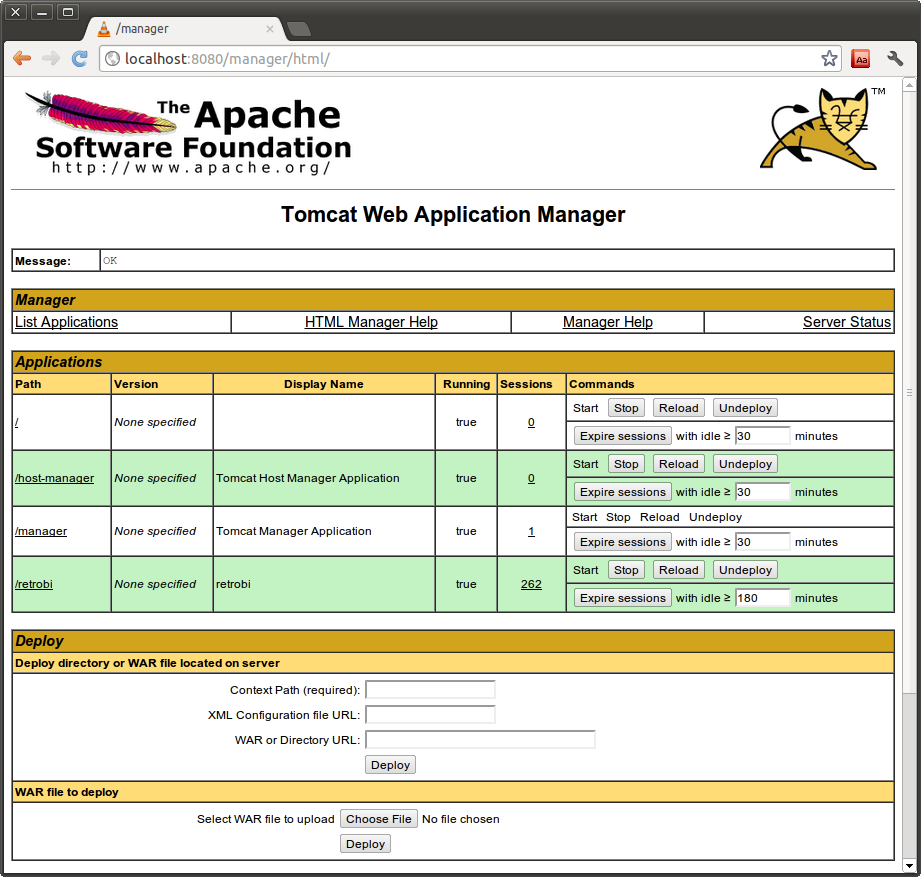
\includegraphics[width=\textwidth]{tomcat.png}
\caption{ovládací konzole serveru Tomcat}
\label{fig:tomcat}
\end{figure}

Více podrobností o možnostech instalace a spouštění aplikací v serveru Tomcat lze najít na této adrese:

\begin{verbatim}
http://tomcat.apache.org/tomcat-7.0-doc/manager-howto.html
\end{verbatim}
